\documentclass[12pt]{article}

\usepackage[a4paper,margin=1in]{geometry}
\usepackage{setspace}
\usepackage{graphicx}
\usepackage{booktabs}
\usepackage{threeparttable}
\usepackage{array}
\usepackage{float}
\usepackage{caption}
\usepackage{subcaption}
\usepackage{hyperref}
\usepackage[round,authoryear]{natbib}

\onehalfspacing
\graphicspath{{figures/}}

\title{Release-Structured, Revision-Aware Real-Time Nowcasting of U.S. GDP}
\author{Ha Minh}
\date{\today}

\begin{document}

\maketitle

\begin{abstract}
This paper studies whether real-time U.S. GDP nowcasts improve when the forecasting system treats GDP as a sequence of official releases rather than as a single final target. The empirical design builds a release ladder for headline real GDP growth using advance, second, third, and mature-vintage targets, denoted $A/S/T/M$, and evaluates forecasts at release-specific real-time information sets. The model comparison includes release-specific autoregressions, bridge regressions, a standard dynamic factor model, a release-structured dynamic factor model, and a revision-aware extension. The main evidence is deliberately conservative. Structured models are most useful for the second and third GDP releases, where the release-structured and revision-aware specifications deliver the lowest headline RMSEs in the frozen evaluation build. The advance release remains difficult: bridge and standard factor benchmarks are highly competitive and often outperform the structured models before the first GDP release. Exact event-time snapshots add value in selected settings, especially near the third release, but the gains are not uniform. Revision forecasts contain useful information about early release revisions, although directional accuracy remains modest. The findings support the value of modeling the GDP release structure in a disciplined real-time pipeline, while cautioning against claims of universal dominance by any single model.
\end{abstract}

\noindent \textbf{Keywords:} GDP nowcasting; real-time data; data revisions; dynamic factor models; release calendar; forecast evaluation.

\noindent \textbf{JEL codes:} C32; C53; E17.

\section{Introduction}

Macroeconomic forecasts are made in real time, but the data used to evaluate those forecasts are not fixed in real time. U.S. GDP is a leading example. The Bureau of Economic Analysis first publishes an advance estimate shortly after the end of the quarter, followed by second and third estimates as additional source data become available. Later vintages can differ materially from the early releases. For forecasters, policy analysts, and financial-market participants, the object being forecast is therefore not only GDP growth but also the specific GDP release that will be observed at a specific date.

Most applied nowcasting systems handle ragged-edge monthly data carefully, but many empirical comparisons still collapse the GDP target into a single quarterly series. That convention is useful for many purposes, but it obscures a core feature of real-time GDP measurement: the second and third GDP releases are not independent forecasting targets. They are updates along a release ladder. They inherit information from the advance release, incorporate new source data, and partly reflect predictable revision dynamics.

This paper asks whether explicitly modeling the release structure improves real-time GDP nowcasting. The analysis uses a reproducible pipeline based on real-time vintages and release-specific forecast origins. The empirical target is headline U.S. real GDP growth. The main GDP release targets are the advance release $A$, the second release $S$, the third release $T$, and a mature-vintage anchor $M$. The core evaluation focuses on $A/S/T$, while $M$ anchors the measurement system and robustness checks. The revision targets are $\Delta_{SA}=S-A$, $\Delta_{TS}=T-S$, and $\Delta_{MT}=M-T$.

The central contribution is not a claim that a complex model dominates at every point in the release cycle. The evidence is more specific. Before the advance release, the information set is still incomplete and simple bridge or standard factor benchmarks remain strong. Before the second and third releases, however, a release-structured representation of the GDP measurement ladder becomes valuable. In the frozen headline evaluation, the release-structured model is the best exact real-time model for the second release, while the revision-aware model is the best model for the third release. The same model family remains important under pandemic exclusion, post-global-financial-crisis subsamples, expanded-panel scenarios, and alternative-data-choice scenarios, although the exact winning model changes across robustness checks.

The paper is organized as follows. Section \ref{sec:literature} positions the project in the nowcasting, real-time data, and data revision literatures. Section \ref{sec:data} describes the data design and real-time snapshot construction. Section \ref{sec:methodology} presents the benchmark and structured models. Section \ref{sec:evaluation} defines the evaluation design. Section \ref{sec:results} reports the main results. Section \ref{sec:robustness} summarizes robustness checks. Section \ref{sec:limitations} discusses limitations. Section \ref{sec:conclusion} concludes.

\section{Related Literature}
\label{sec:literature}

This paper builds on four related literatures. First, it follows the nowcasting literature that treats mixed-frequency, ragged-edge macroeconomic data as a central empirical challenge. \citet{giannone2008} show how the real-time informational content of macroeconomic releases can be evaluated through forecast updates. \citet{mariano2003} provide the classic link between monthly latent activity and quarterly GDP. \citet{banbura2014} provide the estimation reference for dynamic factor models with arbitrary missing-data patterns, which is essential for real-time panels with irregular release timing.

Second, the paper follows the real-time data literature. \citet{croushore2001,croushore2003} emphasize that macroeconomic evaluation can be misleading when revised data are used as if they were available to forecasters in real time. \citet{koenig2003} similarly show that real-time data discipline matters for forecasting comparisons. The present project operationalizes that discipline by constructing event-level release records and snapshot panels at forecast origins.

Third, the paper connects to work on data revisions as a measurement problem. \citet{jacobs2011} model data revisions as a combination of measurement error and dynamics in the underlying true value. This perspective motivates the revision-aware extension: GDP releases are treated as noisy and structured measurements of an underlying quarterly activity state rather than as interchangeable observations.

Fourth, the closest applied motivation is the release- and revision-aware nowcasting work by \citet{anesti2022}. The present paper adapts that logic to a transparent U.S. GDP pipeline, with explicit separation between exact event-time snapshots and pseudo real-time snapshots, and with robustness checks designed for applied macroeconomic journal evaluation.

\section{Data and Real-Time Design}
\label{sec:data}

\subsection{GDP Release Targets}

The target variable is headline U.S. real GDP growth under the BEA release convention. The target system distinguishes four release concepts: $A$ is the advance GDP release, $S$ is the second GDP release, $T$ is the third GDP release, and $M$ is the mature GDP vintage, implemented as the 12-quarter-later vintage. The main evaluation tables focus on $A/S/T$ because these are the releases faced by real-time users. The mature target $M$ is retained as an anchor for the latent measurement system and for robustness analysis.

Revision targets are defined as:
\begin{equation}
\Delta_{SA}=S-A,\quad \Delta_{TS}=T-S,\quad \Delta_{MT}=M-T.
\end{equation}

The source-of-truth build for this manuscript is the frozen artifact directory \texttt{outputs/frozen/submission\_final}. Every number reported in the paper is traceable to a CSV in that directory.

\subsection{Monthly Indicator Panel}

The monthly information set is designed around a core panel of real-time U.S. indicators. The panel covers labor markets, production, spending and housing, trade and inventories, financial conditions, and survey information. Indicators are transformed using pre-specified stationarity transformations and standardized with expanding-window moments so that information after the forecast origin is not used.

The implementation prioritizes reproducibility over breadth. Adding many indicators without reliable vintage timing can improve in-sample fit while weakening the real-time validity of the exercise. The paper therefore treats the core panel as the primary design and reports expanded-panel and alternative-data-choice scenarios as robustness checks rather than as the headline specification.

\subsection{Exact and Pseudo Real-Time Snapshots}

The pipeline constructs two timing designs. The exact design uses event-level public release timestamps when available and applies agency-specific timestamp assumptions when historical files provide release dates but not release times. The pseudo design uses a coarser timing convention. Comparing the two designs provides a direct test of whether exact release timing materially changes forecast performance.

The exact timing comparison is not expected to dominate in every cell. The empirical question is narrower: whether event-time discipline matters at economically relevant release checkpoints. In the frozen results, exact timing is most useful for selected later-release cases, especially the third-release structured models.

\subsection{Census Proxy Limitation}

One data caveat is important for interpretation. The current build does not use a full historical official Census release archive for every relevant Census series. Instead, some Census-sensitive timing is proxied through first-release information available in the real-time data pipeline. This is a defensible operational solution for a reproducible pipeline, but it must be disclosed clearly. The robustness section therefore includes alternative-data-choice checks to test whether the main story is overly dependent on that proxy.

\section{Methodology}
\label{sec:methodology}

The model set is intentionally tiered. The paper first establishes simple benchmarks, then introduces structured models that encode the GDP release ladder.

\subsection{Release-Specific Autoregression}

The autoregressive benchmark estimates separate models for each GDP release target. Lag order is selected from one to four lags by BIC in an expanding-window design. This benchmark tests whether monthly indicators and release-structure information add value beyond the target's own history.

\subsection{Bridge Regression}

The bridge model summarizes the monthly indicator panel into block-level features and maps those features into quarterly GDP release targets through expanding-window OLS. Missing within-quarter monthly observations are nowcast with univariate autoregressions for the relevant indicators. This benchmark is important for the advance release because it can be highly competitive when the first GDP estimate depends heavily on incomplete monthly source data.

\subsection{Standard Dynamic Factor Model}

The standard dynamic factor model uses a common monthly factor extracted from the real-time indicator panel, with a simple quarterly aggregation link to GDP. It is estimated separately for each GDP release target. This model provides a conventional factor-model benchmark: it uses mixed-frequency information but does not explicitly model the release ladder across $A/S/T/M$.

\subsection{Release-Structured Dynamic Factor Model}

The release-structured dynamic factor model introduces a shared latent quarterly activity state and separate measurement equations for the GDP release targets $A/S/T/M$. The design recognizes that GDP releases are related measurements of the same underlying quarterly activity concept. The model is therefore allowed to learn release-specific measurement behavior while retaining a common activity signal.

This is the first contribution model in the paper. It is not designed to win at every checkpoint. Its expected advantage is strongest after at least one GDP release has been observed, because later releases contain both new source data and information about the earlier release.

\subsection{Revision-Aware Dynamic Factor Model}

The revision-aware extension adds a parsimonious latent revision component to the release-structured system. The revision state follows a simple dynamic process and is anchored so that the mature vintage is treated as the reference point. The purpose is to capture predictable components of early GDP revisions without building a full joint revision system for every monthly indicator.

This model is structural for the GDP release ladder, not for all source-data revisions. The current paper asks whether GDP release revisions contain forecastable structure. It does not claim to solve the broader problem of fully modeling revisions across the entire macroeconomic indicator panel.

\section{Forecast Evaluation Design}
\label{sec:evaluation}

The evaluation sample is 2005Q1--2024Q4, with 80 quarterly forecast targets in the headline tables. Earlier observations are used for burn-in and model estimation. The main release checkpoints are \texttt{pre\_advance}, the day before the advance GDP release; \texttt{pre\_second}, the day before the second GDP release; and \texttt{pre\_third}, the day before the third GDP release.

Models are evaluated using RMSE, MAE, bias, relative RMSFE, Diebold-Mariano comparisons, small-sample adjusted Diebold-Mariano comparisons, and sign accuracy where applicable. The paper interprets statistical tests conservatively because the sample is finite, the forecast origins are structured by release timing, and the robustness results show that exact model winners are not fully stable across subsamples.

\section{Empirical Results}
\label{sec:results}

\subsection{Headline Point Forecasts}

Table \ref{tab:headline} summarizes the headline winners from the frozen point-forecast results. The full generated table is stored in \texttt{paper/tables/table\_1\_headline\_point\_forecasts.md}, and the source CSV is \texttt{outputs/frozen/submission\_final/headline\_point\_results.csv}.

\begin{table}[!htbp]
\centering
\begin{threeparttable}
\caption{Headline winners by target and snapshot mode}
\label{tab:headline}
\small
\begin{tabular}{lllllp{5.2cm}}
\toprule
Snapshot & Target & Checkpoint & Best model & RMSE & Interpretation \\
\midrule
exact & $A$ & pre-advance & bridge & 5.151 & Advance GDP remains difficult; the bridge benchmark is strongest. \\
exact & $S$ & pre-second & release DFM & 0.669 & Release-structured modeling is strongest for the second release. \\
exact & $T$ & pre-third & revision DFM & 0.364 & Revision-aware modeling is strongest for the third release. \\
pseudo & $A$ & pre-advance & standard DFM & 5.065 & A conventional factor benchmark is strongest under pseudo timing. \\
pseudo & $S$ & pre-second & revision DFM & 0.667 & Structured models dominate the second-release comparison. \\
pseudo & $T$ & pre-third & revision DFM & 0.388 & Revision-aware modeling remains strongest for the third release. \\
\bottomrule
\end{tabular}
\begin{tablenotes}
\footnotesize
\item Source: \texttt{outputs/frozen/submission\_final/headline\_point\_results.csv}. Lower RMSE is better.
\end{tablenotes}
\end{threeparttable}
\end{table}

The main result is clear but should be stated carefully. The release-structured and revision-aware models are not uniformly best at the advance release. In both exact and pseudo timing designs, the strongest advance-release models are simpler benchmarks: bridge under exact timing and standard DFM under pseudo timing. The structured models perform much better for $S$ and $T$, where the release ladder becomes directly informative.

The size of the later-release gains is large in the frozen build. Under exact timing, the best $S$ model has RMSE 0.669 and the best $T$ model has RMSE 0.364, compared with much higher errors for the simple autoregressive benchmark. This does not mean the model has solved advance GDP forecasting. It means the model uses the information embedded in the release sequence effectively once earlier GDP release information is available.

\subsection{Exact-vs-Pseudo Timing}

Table \ref{tab:timing} reports the exact-minus-pseudo RMSE gaps for the structured models. The full timing comparison is stored in \texttt{paper/tables/table\_2\_exact\_vs\_pseudo.md}, and the source CSV is \texttt{outputs/frozen/submission\_final/headline\_exact\_vs\_pseudo.csv}.

\begin{table}[!htbp]
\centering
\begin{threeparttable}
\caption{Exact-minus-pseudo RMSE gaps for structured models}
\label{tab:timing}
\small
\begin{tabular}{llrrr}
\toprule
Target & Model & Exact RMSE & Pseudo RMSE & Exact minus pseudo \\
\midrule
$A$ & release DFM & 7.379 & 7.363 & 0.016 \\
$A$ & revision DFM & 7.309 & 7.294 & 0.015 \\
$S$ & release DFM & 0.669 & 0.668 & 0.000 \\
$S$ & revision DFM & 0.671 & 0.667 & 0.005 \\
$T$ & release DFM & 0.370 & 0.392 & -0.023 \\
$T$ & revision DFM & 0.364 & 0.388 & -0.024 \\
\bottomrule
\end{tabular}
\begin{tablenotes}
\footnotesize
\item Source: \texttt{outputs/frozen/submission\_final/headline\_exact\_vs\_pseudo.csv}. Negative gaps indicate lower RMSE under exact event-time snapshots.
\end{tablenotes}
\end{threeparttable}
\end{table}

Exact timing does not mechanically improve every forecast. For the advance release, the exact structured models are slightly worse than pseudo timing. For the second release, the difference is negligible. For the third release, however, exact timing improves both structured specifications. This pattern is consistent with the paper's broader interpretation: timing discipline is most useful when the release ladder and event sequence are most informative.

\subsection{Revision Forecasts}

Table \ref{tab:revision} reports revision-target forecasts. The full table is stored in \texttt{paper/tables/table\_3\_revision\_forecasts.md}, and the source CSV is \texttt{outputs/frozen/submission\_final/headline\_revision\_results.csv}.

\begin{table}[!htbp]
\centering
\begin{threeparttable}
\caption{GDP release-revision forecasting performance}
\label{tab:revision}
\small
\begin{tabular}{llllrrrr}
\toprule
Snapshot & Revision target & Checkpoint & Model & RMSE & MAE & Bias & Sign accuracy \\
\midrule
exact & $\Delta_{SA}$ & pre-advance & revision DFM & 0.570 & 0.400 & 0.066 & 0.392 \\
pseudo & $\Delta_{SA}$ & pre-advance & revision DFM & 0.570 & 0.400 & 0.066 & 0.392 \\
exact & $\Delta_{TS}$ & pre-second & revision DFM & 0.361 & 0.238 & 0.054 & 0.405 \\
pseudo & $\Delta_{TS}$ & pre-second & revision DFM & 0.370 & 0.242 & 0.063 & 0.405 \\
\bottomrule
\end{tabular}
\begin{tablenotes}
\footnotesize
\item Source: \texttt{outputs/frozen/submission\_final/headline\_revision\_results.csv}. Revision forecasts are supporting evidence rather than the central model-dominance claim.
\end{tablenotes}
\end{threeparttable}
\end{table}

The revision results should be treated as supporting evidence. The model produces lower RMSE for $\Delta_{TS}$ than for $\Delta_{SA}$, and exact timing helps slightly for $\Delta_{TS}$. However, sign accuracy is only modest. The evidence supports the presence of forecastable magnitude information in early revisions, but it does not justify a strong claim that revision directions are reliably predicted.

\subsection{Forecast Update Figures}

Figures \ref{fig:nowcast} and \ref{fig:decomp} show the nowcast path and the forecast update decomposition from the frozen reporting pipeline.

\begin{figure}[!htbp]
\centering
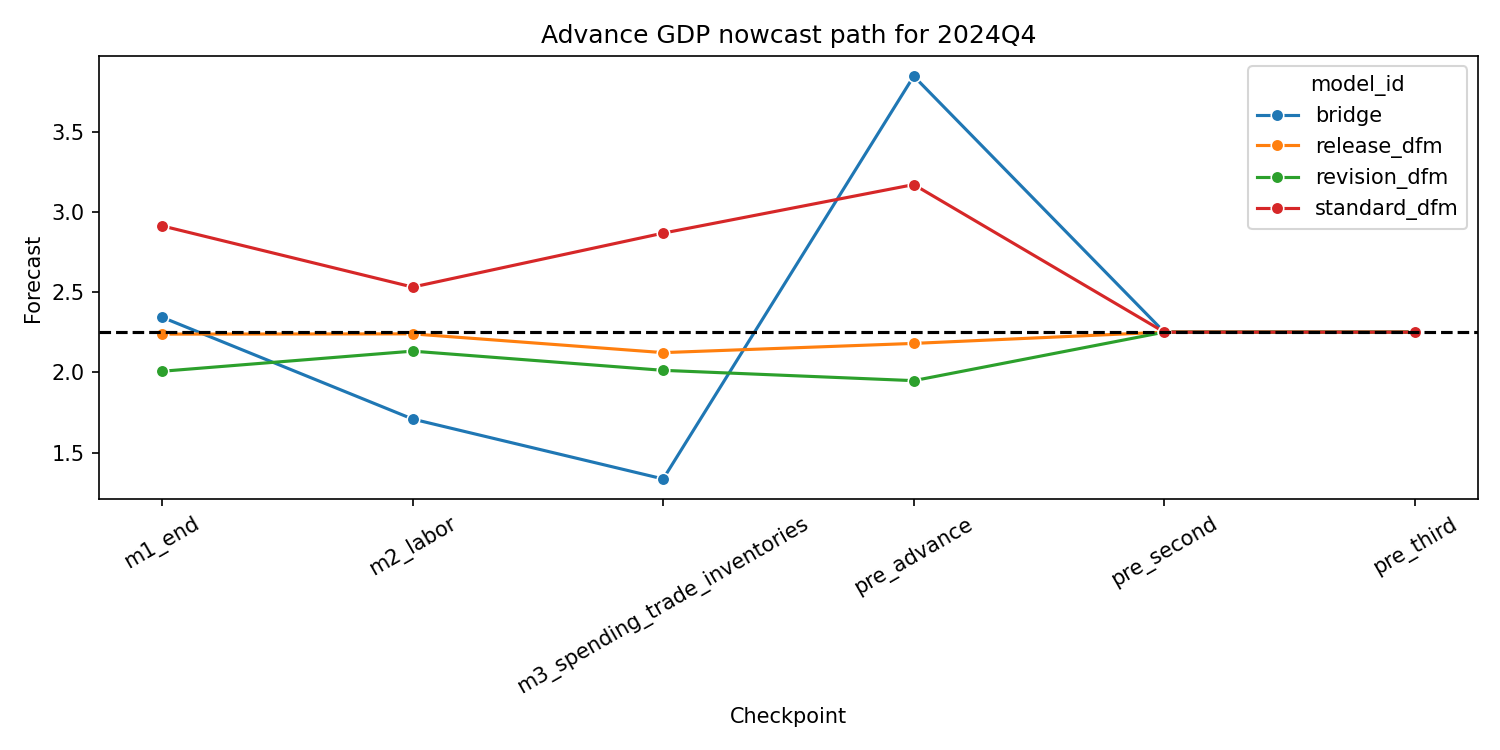
\includegraphics[width=0.88\textwidth]{nowcast_path.png}
\caption{Nowcast path across release checkpoints}
\label{fig:nowcast}
\end{figure}

\begin{figure}[!htbp]
\centering
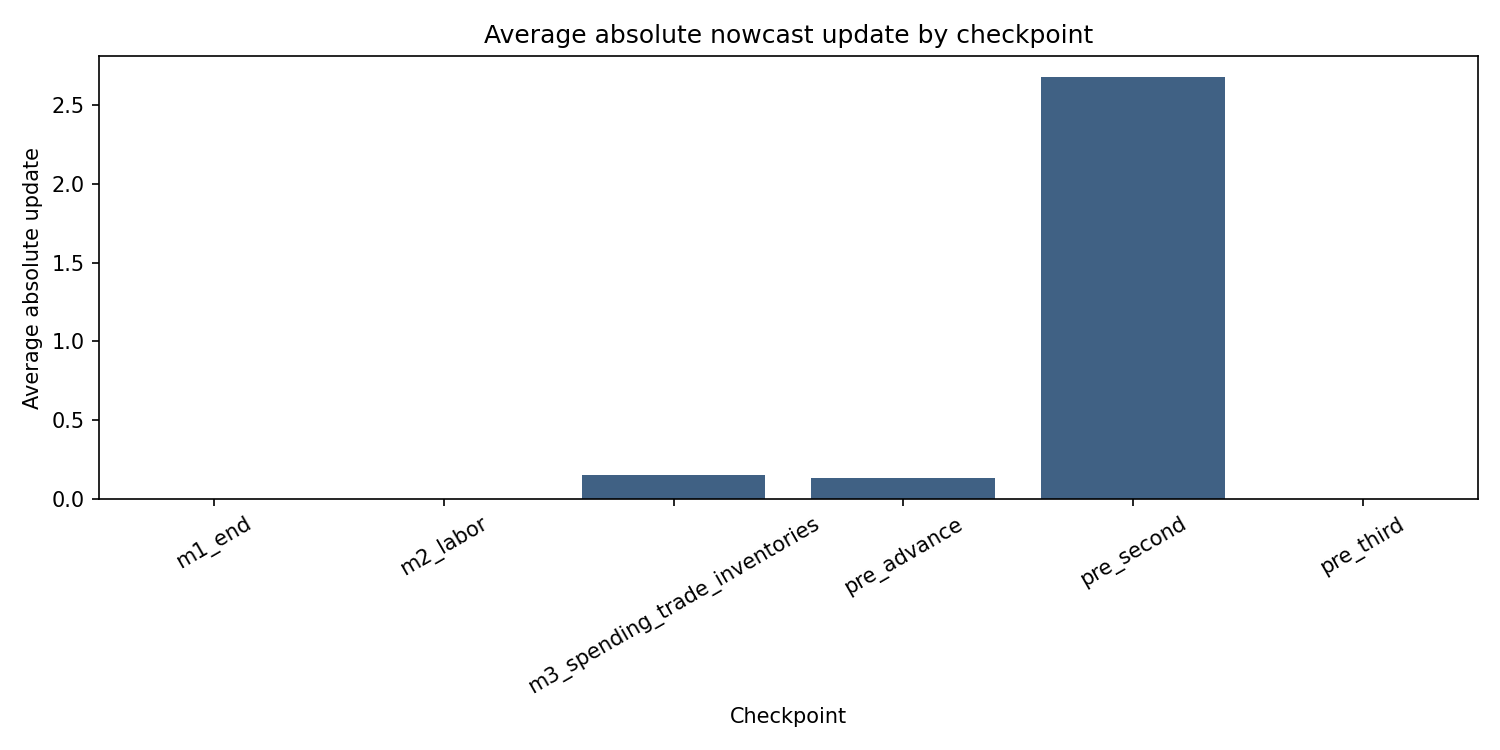
\includegraphics[width=0.88\textwidth]{forecast_update_decomposition.png}
\caption{Forecast update decomposition across checkpoints}
\label{fig:decomp}
\end{figure}

Figure \ref{fig:nowcast} is useful for showing how the nowcast evolves as the information set approaches the GDP release dates. Figure \ref{fig:decomp} is useful for explaining why the release-structured design matters: it separates forecast movements across checkpoints rather than treating the GDP target as a single static object.

\section{Robustness}
\label{sec:robustness}

The robustness strategy is designed to protect the central claim rather than to search for a universal winner. The source files are \texttt{headline\_point\_subsample\_robustness.csv}, \texttt{headline\_point\_scenario\_robustness.csv}, \texttt{headline\_point\_small\_sample\_dm.csv}, and \texttt{journal\_winner\_stability.csv} in the frozen result folder.

Table \ref{tab:robustness} summarizes the exact-timing winners across key robustness checks. The full generated robustness tables are stored in \texttt{paper/tables/table\_4\_robustness\_winners.md}, \texttt{paper/tables/appendix\_a\_subsample\_robustness\_full.md}, and \texttt{paper/tables/appendix\_a\_scenario\_robustness\_full.md}.

\begin{table}[!htbp]
\centering
\begin{threeparttable}
\caption{Exact-timing robustness winners}
\label{tab:robustness}
\small
\begin{tabular}{llllp{5.6cm}}
\toprule
Robustness check & $A$ winner & $S$ winner & $T$ winner & Interpretation \\
\midrule
Alternative data choice & bridge & release DFM & revision DFM & Structured models remain best for $S/T$. \\
Expanded panel & standard DFM & revision DFM & release DFM & Structured model family remains best for $S/T$. \\
Exclude pandemic quarters & bridge & release DFM & revision DFM & The main $S/T$ pattern survives pandemic exclusion. \\
Post-GFC sample & bridge & release DFM & revision DFM & The main $S/T$ pattern survives the larger post-GFC subsample. \\
Pre-GFC sample & release DFM & release DFM & release DFM & Results are supportive but based on only 12 forecasts. \\
\bottomrule
\end{tabular}
\begin{tablenotes}
\footnotesize
\item Sources: \texttt{headline\_point\_subsample\_robustness.csv} and \texttt{headline\_point\_scenario\_robustness.csv}.
\end{tablenotes}
\end{threeparttable}
\end{table}

The robustness evidence supports a model-family claim, not a single-model dominance claim. The winner-stability file shows that \texttt{winner\_is\_stable} is false for every target and snapshot-mode pair. This instability is not fatal because the paper's main claim is not that \texttt{revision\_dfm} always wins. The defensible claim is that structured models are consistently important for the second and third releases, while the advance release is harder and remains highly sensitive to model choice and sample design.

The pandemic exclusion check is especially important. Excluding the pandemic quarters sharply reduces advance-release RMSE for simpler models, illustrating how much the advance-release comparison is affected by extreme observations. The second and third release findings remain aligned with the structured-model story.

Small-sample Diebold-Mariano results should be interpreted cautiously. The reported p-values for structured-model gains in the main $S/T$ cells are informative but not overwhelmingly small. This is another reason the paper should emphasize economic and real-time design relevance rather than overstate statistical dominance.

\section{Limitations}
\label{sec:limitations}

The first limitation is data timing. The pipeline has event-level timestamps and applies real-time leakage tests, but some Census-sensitive historical timing relies on a first-release proxy rather than a complete official Census historical release archive. This limitation is partially addressed by alternative-data-choice robustness checks, but it remains a disclosure point for journal submission.

The second limitation is the advance-release result. The structured models do not dominate before the advance GDP release. This is not a weakness to hide. It is an important empirical finding: before the first GDP estimate, the available monthly data and bridge-style aggregation remain highly competitive.

The third limitation is the scope of the revision-aware model. The model is revision-aware for the GDP release ladder, not for the full monthly indicator panel. A full joint system with indicator revisions, GDP revisions, and density forecasts would be more comprehensive but also substantially more complex.

The fourth limitation is sample size. The main evaluation has 80 quarterly forecasts, and subsample tests can become small, especially pre-GFC. This motivates conservative interpretation of forecast comparison tests.

The fifth limitation is external validity. The model is designed around the U.S. GDP release system. The same logic can be applied to other countries, but the release calendar, source-data structure, and revision process would need to be rebuilt.

\section{Conclusion}
\label{sec:conclusion}

This paper shows that release structure matters for real-time GDP nowcasting, but not in a simplistic way. The advance release remains the hardest stage of the GDP release ladder, and conventional bridge or factor benchmarks can be the best models before that first official estimate. The value of the structured approach is clearest before the second and third GDP releases, where earlier GDP releases and revision dynamics become part of the relevant real-time information set.

The empirical contribution is therefore twofold. First, the paper provides a reproducible real-time pipeline that distinguishes advance, second, third, and mature GDP targets and evaluates forecasts at release-specific origins. Second, it shows that release-structured and revision-aware factor models are practically useful for later GDP releases, even though exact model winners vary across robustness designs.

The next research step is not to add complexity indiscriminately. The most valuable extensions are targeted: improve official Census release timing, add a carefully scoped monthly-indicator revision block, and develop density forecasts around the release ladder. These extensions would strengthen the framework while preserving the paper's central discipline: every forecast must respect the information actually available at the forecast origin.

\appendix

\section{Additional Timing Figure}

\begin{figure}[H]
\centering
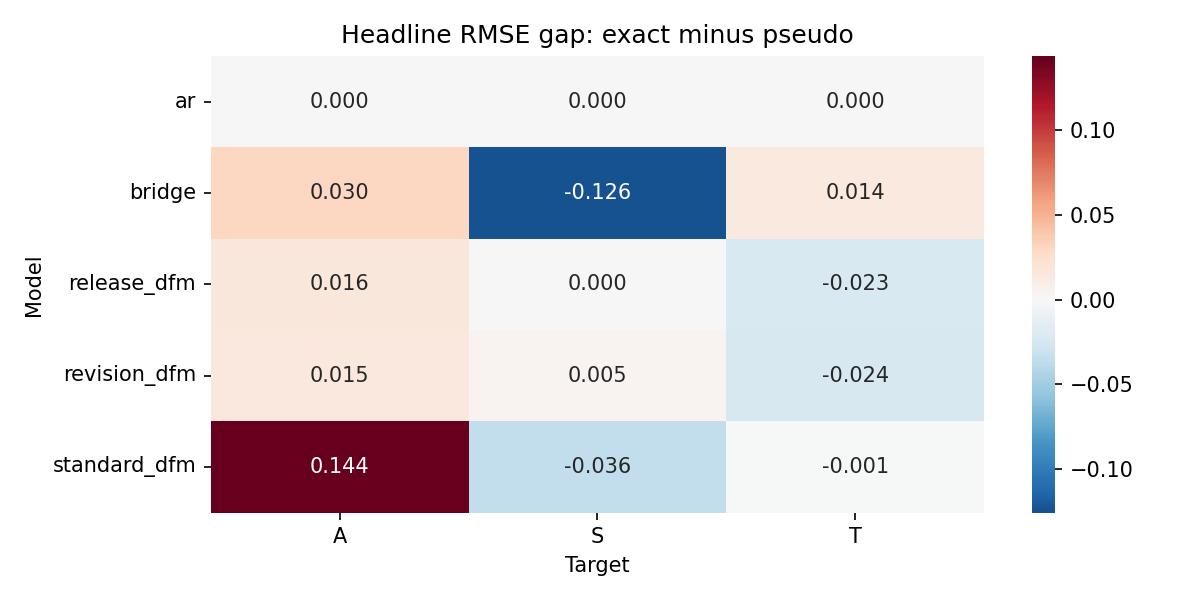
\includegraphics[width=0.88\textwidth]{submission_exact_vs_pseudo_gap.png}
\caption{Exact-vs-pseudo RMSE gaps}
\label{fig:exactpseudo}
\end{figure}

\section{Reproducibility Note}

All numerical results in this manuscript come from \texttt{outputs/frozen/submission\_final}. The generated paper tables are stored in \texttt{paper/tables}. The manuscript should not be edited using numbers from older output folders unless a new freeze is created and explicitly documented.

\begin{thebibliography}{99}

\bibitem[Anesti et~al.(2022)]{anesti2022}
Anesti, N., Galvao, A.~B., and Miranda-Agrippino, S. (2022).
\newblock Uncertain Kingdom: Nowcasting GDP and its revisions.
\newblock \emph{Journal of Applied Econometrics}, 37(1), 42--62.

\bibitem[Banbura and Modugno(2014)]{banbura2014}
Banbura, M. and Modugno, M. (2014).
\newblock Maximum likelihood estimation of factor models on datasets with arbitrary pattern of missing data.
\newblock \emph{Journal of Applied Econometrics}, 29(1), 133--160.

\bibitem[Croushore and Stark(2001)]{croushore2001}
Croushore, D. and Stark, T. (2001).
\newblock A real-time data set for macroeconomists.
\newblock \emph{Journal of Econometrics}, 105(1), 111--130.

\bibitem[Croushore and Stark(2003)]{croushore2003}
Croushore, D. and Stark, T. (2003).
\newblock A real-time data set for macroeconomists: Does data vintage matter?
\newblock \emph{Review of Economics and Statistics}, 85(3), 605--617.

\bibitem[Giannone et~al.(2008)]{giannone2008}
Giannone, D., Reichlin, L., and Small, D. (2008).
\newblock Nowcasting: The real-time informational content of macroeconomic data.
\newblock \emph{Journal of Monetary Economics}, 55(4), 665--676.

\bibitem[Jacobs and van Norden(2011)]{jacobs2011}
Jacobs, J.~P.~A.~M. and van Norden, S. (2011).
\newblock Modeling data revisions: Measurement error and dynamics of true values.
\newblock \emph{Journal of Econometrics}, 161(2), 101--109.

\bibitem[Koenig et~al.(2003)]{koenig2003}
Koenig, E.~F., Dolmas, S., and Piger, J. (2003).
\newblock The use and abuse of real-time data in economic forecasting.
\newblock \emph{Review of Economics and Statistics}, 85(3), 618--628.

\bibitem[Mariano and Murasawa(2003)]{mariano2003}
Mariano, R.~S. and Murasawa, Y. (2003).
\newblock A new coincident index of business cycles based on monthly and quarterly series.
\newblock \emph{Journal of Applied Econometrics}, 18(4), 427--443.

\end{thebibliography}

\end{document}
